\documentclass{beamer}
\usetheme{PaloAlto}
\usepackage[croatian]{babel}

\usepackage{animate}

\setbeamertemplate{caption}[numbered]
\usepackage{listings}
\usepackage{amsmath}
\PassOptionsToPackage{height=1.5cm}{beamerouterthemesidebar}
\usefonttheme[]{structurebold}

\usepackage{multirow}
 
\setbeamertemplate{page number in head/foot}[totalframenumber]
\setbeamertemplate{navigation symbols}{\footnotesize\usebeamertemplate{page number in head/foot}}

\usepackage{xcolor}

\definecolor{myblue}{RGB}{50, 151, 212}
\usecolortheme[named=myblue]{structure}
\setbeamerfont{frametitle}{size=\large,series=\bfseries,shape=\itshape}
\usepackage[utf8]{inputenc}
\title{Programming language Pharo}
\author{Lucija Žužić, Barbara Breš, Mihael Petranović, Borna Sila, Dorijan Janžetič, Vedran Matić}
\institute[]{Tehnički Fakultet Sveučilište u Rijeci\newline Preddiplomski sveučilišni studij računarstva,  Programsko inženjerstvo}
\date{2. ožujka 2021.}



\begin{document}
\logo{
\includegraphics[width=0.1\linewidth]{icone-pharo-1.png}}
\titlegraphic{
\includegraphics[width=0.5\linewidth]{pharo.png}}
\maketitle
\section{Značajke}
\begin{frame}{Značajke (prvi dio)}
\begin{itemize}
    \item Optional fusion of developed program and development environment
    \item A pure object-oriented approach
    \item Simple syntax
    \item Immediate object identity swapping
    \item Resumable exceptions
    \item Live object inspection
    \item Dynamic inheritance
    \item Multiplatform virtual machine with JIT, combined generational \item garbage collector, ephemerons, forwarders
    \item Easy call stack manipulation
\end{itemize}
\end{frame}
\begin{frame}{Značajke (drugi dio)}
\begin{itemize}
    \item Fast object enumeration
    \item Objects as methods
    \item Optional Green threads
    \item AST metalinks
    \item Customizable metaclasses
    \item Relatively low memory consumption
    \item Customizable compiler
    \item Optional complete object memory persistence
    \item Fast object serialization
    \item Easy use of proxy objects
\end{itemize}
\end{frame}

\begin{frame}{Opcionalno spajanje razvijenog programa i razvojne okoline}
%\includegraphics[width=0.5\linewidth]{fusion.gif}
%\frame{\inlineMovie[loop&autostart&start=1]{fusion.avi}{}{height=0.7\textheight}}
\begin{itemize}
    \item U jeziku Pharo, granica između programa i IDE-a se može eliminirati. To znači da se kod može izravno koristiti za vizualno predstavljanje struktura podataka tijekom debugiranja te se ugrađeni alati mogu lako modificirati da odgovaraju vašim potrebama itd.
\end{itemize}
\begin{block}{}

On a breakpoint, use the custom circuit region visual representation in the debugger, run another debugger on a piece of code inside the original debugger, edit the circuit inside the debugger and continue in stepping
\end{block}
\end{frame}

\begin{frame}{Advanced run-time reflection}
%\includegraphics[width=0.5\linewidth]{pointers.gif}
%\frame{\inlineMovie[loop&autostart&start=1]{pointers.avi}{}{height=0.7\textheight}}
\begin{itemize}
    \item Pharo sve otkriva programeru. Svaki objekt u sustavu se može pregledati i izmijeniti s obzirom na pravila enkapsulacije (učahurivanja).
    \item Pharo može enumerirati sve objekte koji imaju reference na neki objekt.
    Pharo exposes everything to the programmer. Every object in the system can be examined and changed with respect to the object encapsulation rules.
    \item Pharo can enumerate all objects that have reference to some object.
\end{itemize}
\begin{block}{}
Open inspector on some window instance, find all objects that have reference to it and investigate them
\end{block}
\end{frame}

\begin{frame}{Čisti objektno orijentirani pristup}
%\includegraphics[width=0.5\linewidth]{oop.gif}
\begin{itemize}
    \item U jeziku Pharo, sve je objekt. Ova čistoća i uniformnost u sustavu i dizajnu jezika čine Pharo ugodnim za učenje. In Pharo, everything is an object. This purity and uniformity in the system and language design makes Pharo clean and comfortable to learn.
\end{itemize}
\begin{block}{}
True is instance of the class named True that has methods for control structures (like ifTrue:) that work with closures
True je instanca klase true koja ima metode za kontrolne strukture (poput ifTrue:) 
\end{block}
\end{frame}

\begin{frame}{Software as objects}
%\includegraphics[width=0.5\linewidth]{navigation.gif}
\begin{itemize}
    \item Pharo uses files for serialization of source code, but, by default, it does not use files to edit them. Instead of a text editor, it provides the tools to browse and modify the classes, methods, class comments and other program entities. So Pharo has a much better understanding of relations between them and allows easier navigation and refactorings.
\end{itemize}
\begin{block}{}
Find all references to a class, all method implementors and senders
\end{block}
\end{frame}

\begin{frame}{Jednostavna sintaksa jezika}
\begin{itemize}
    \item Sintaksa ima samo 6 rezerviranih ključnih riječi
    \item Gramatika je LL(1) pa je vrlo brz za parsiranje
    \item Jednostavan za učenje
    \item Pharo je dizajniran za prosljeđivanje poruka bez dvosmislenosti argumenata
\end{itemize}

\begin{figure}
    \centering
    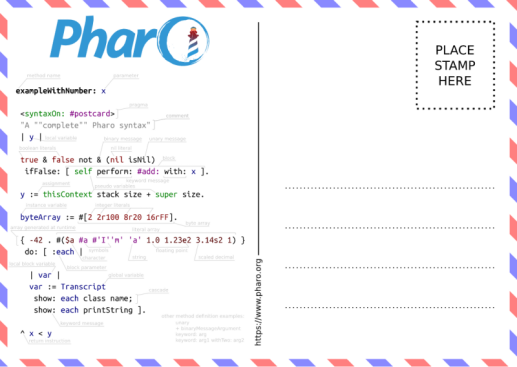
\includegraphics[width=0.8\linewidth]{postcard.png}
    \label{fig:postcard}
    \caption{Svi elementi jezika koji se nalaze u Pharu stanu na jednu razglednicu}
\end{figure}
\end{frame}

\begin{frame}{Closures with non-local returns}
\begin{itemize}
    \item The closures in Pharo with non-local returns allow elegant implementation of control structures without needing to define them in the language itself. Pharo is a simple meta-language where the programmer has all features required for the writing of custom readable domain-specific languages.
\end{itemize}
\begin{figure}
    \centering
    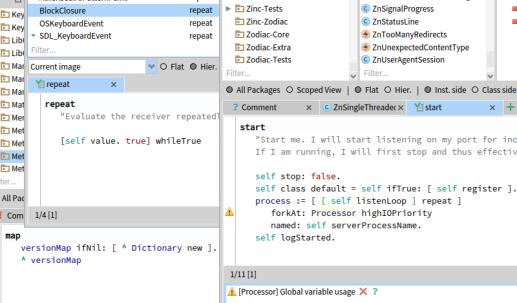
\includegraphics[width=0.8\linewidth]{controlStructures.png}
    \label{fig:controlStructures}
    \caption{Show implementaion and usage of message repeat. A method (map) that contains closure with non-local return}
\end{figure}
\end{frame}

\begin{frame}{Immediate objects identity swapping}
%\includegraphics[width=0.5\linewidth]{become.gif}
\begin{itemize}
    \item In Pharo, you can easily replace an object with another one. All references to the old object in your running program will be replaced by references to the new object.
\end{itemize}
\begin{block}{}
Inspect all graphical elements on desktop, find logo, create new picture from a display region selected by the user and change identity of the logo object to this new picture*
\end{block}
\end{frame}

\begin{frame}{Fast resumable exceptions}
%\includegraphics[width=0.5\linewidth]{exceptions.gif}
\begin{itemize}
    \item Pharo provides advanced exceptions system that can do things like resuming from a raised exception with providing an alternative result so your program can recover from failures.
    \item Their fast speed allows them to be used for clean information-flow mechanisms.
\end{itemize}
\begin{block}{}
Provide an alternative result of the faulty expression that tries the division by zero
\end{block}
\end{frame}

\begin{frame}{Live customizable objects inspection}
%\includegraphics[width=0.5\linewidth]{inspector.gif}
\begin{itemize}
    \item You can visualize your objects in many ways (textual form, graphical representation) and use it to inspect the state of your running program. Debuggers can use these visualizations to help you to your understanding.
\end{itemize}
\begin{block}{}
Inspect an object graph with help of custom interactive visual object representations    
\end{block}
\end{frame}

\begin{frame}{Run-time classes and objects migration}
%\includegraphics[width=0.5\linewidth]{migration.gif}
\begin{itemize}
    \item Pharo can evolve while it’s running. It is like an organism. You can do things like add or remove instance variables of classes that have already existing instances. All these living instances will be properly modified.
\end{itemize}
\begin{block}{}
Look at some random instance of a class and add new variable to this class
\end{block}
\end{frame}

\begin{frame}{Dynamic inheritance}
%\includegraphics[width=0.5\linewidth]{inheritance.gif}

\begin{itemize}
    \item You can change the definition of existing classes including changing its superclass. To some selected object, you can simply assign a different class and do similar operations. These capabilities are essential for the ability of the system to evolve without the need for restarts.
\end{itemize}
\begin{block}{}
Count all living instances of a class Point, create a new class with half of its original variables and use it as new superclass of Point while the graphical system is running
\end{block}

\end{frame}

\begin{frame}{Napredan višeplatformski virtualni stroj sa JIT, kombiniranim generacijskim garbage collectorom, ephemeronima i forwarderima}
\begin{itemize}
    \item Pharo koristi vrlo brzi virtualni stroj s mnogim jedinstvenim mogućnostima i koji se može pokrenuti na Windowsu, macOS-u, Linuxu te na ARM procesorima
\end{itemize}
\begin{figure}
    \centering
    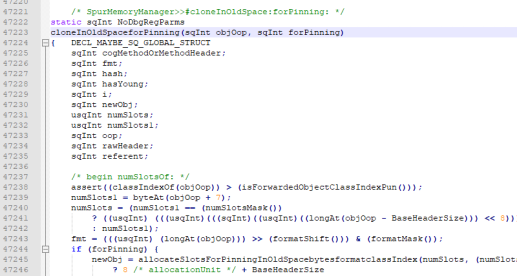
\includegraphics[width=0.8\linewidth]{vm.png}
    \label{fig:vm}
    \caption{Dio izvornog koda garbage collectora koji se bavi pinned objektima koji imaju stabilne lokacije u memoriji}
\end{figure}
\end{frame}

\begin{frame}{Virtualni stroj koji je većinom napisan u samom programskom jeziku Pharo}
\begin{itemize}
    \item Da bi razumijevanje i debugiranje virtualnog stroja bilo prirodnije, većinom je napisan u Pharu.
\end{itemize}
\begin{figure}
    \centering
    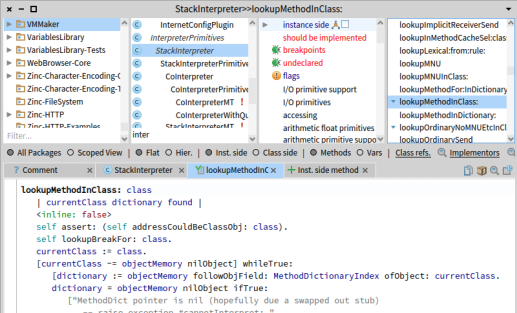
\includegraphics[width=0.8\linewidth]{vmmaker.png}
    \label{fig:vmmaker}
    \caption{Dio izvornog koda garbage collectora koji se bavi pinned objektima koji imaju stabilne lokacije u memoriji}
\end{figure}
\end{frame}

\begin{frame}{Lagana manipulacija stogom poziva}
\begin{itemize}
    \item Lako se može pregledati, izmijeniti ili serijalizirati stog poziva. Ovo omogućava, između ostalog, mnogo jednostaniju izgradnju alata za debugiranje.
\end{itemize}
\begin{figure}
    \centering
    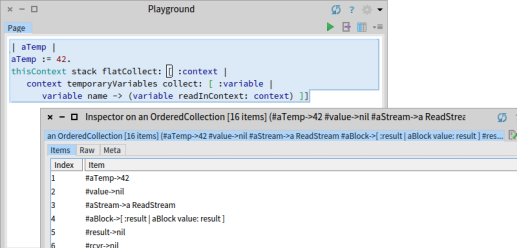
\includegraphics[width=0.8\linewidth]{stack.png}
    \label{fig:stack}
    \caption{Pregledajte sve privremene varijable i njihove vrijednosti u stogu poziva.}
\end{figure}
\end{frame}

\begin{frame}{Continuations}
\begin{itemize}
    \item Call stack manipulation allows surprisingly easy implementation of continuations without the need for direct support of the virtual machine. The continuations are very handy for web development tasks and backtracking implementation.
\end{itemize}
\begin{figure}
    \centering
    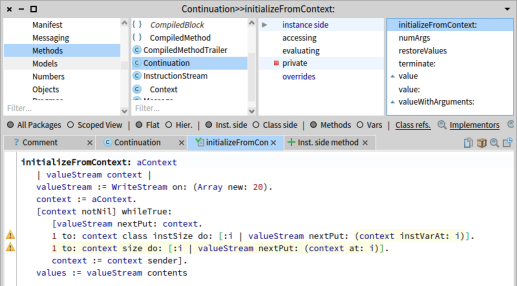
\includegraphics[width=0.8\linewidth]{continuation.png}
    \label{fig:continuation}
    \caption{Continuations are implemented in a very small elegant class.}
\end{figure}
\end{frame}

\begin{frame}{Fast object enumeration}
\begin{itemize}
    \item With the Pharo reflection, you can easily enumerate all existing instances of a particular class and investigate references to them. It is beneficial for detecting memory leaks. It is an essential Pharo reflectivity feature.
\end{itemize}
\begin{block}{}
Find all existing strings that contain subsctring ‘Pharo has’ and visualize them as a tree map according their sizes
\end{block}
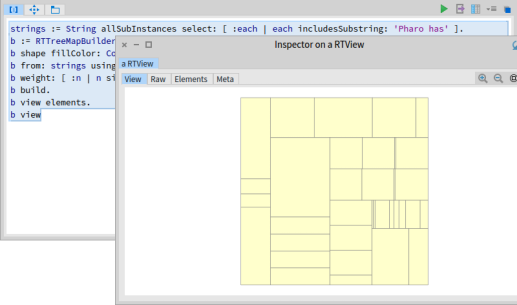
\includegraphics[width=0.5\linewidth]{instances.png}
\end{frame}

\begin{frame}{Objects as methods Objekti kao metode}
\begin{itemize}
    \item Methods are objects and objects can serve as methods. In this case, the invoking of a method means that the object receives a special message. It may be used for example during the coverage testing. You replace all class methods with such proxy objects, and when called, these objects replace themselves with the original method and write this information to a log.
    Metode su objekti i objekti mogu služiti kao metode. U tom slučaju, poziv metode znači da objekt prima posebnu poruku. Ovo se može korisiti, na primjer, za vrijeme coverage testinga. Tada se treba zamijeniti sve metode klasa proxy objektima koji zamijene sami sebe originalnom metodom kada ih pozovemo i zapišu te informacije na stog. 
\end{itemize}
\begin{block}{}
To implement per-method coverage is matter of few lines of code
\end{block}
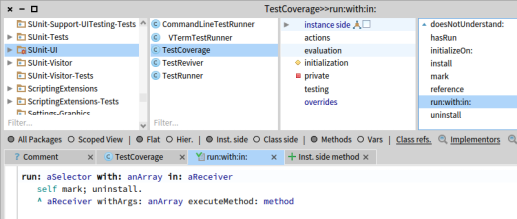
\includegraphics[width=0.5\linewidth]{methods.png}
\end{frame}

\begin{frame}{Traits}
\begin{itemize}
    \item Pharo classes use single inheritance, but they can use stateful traits for sharing of behavior with other classes.
\end{itemize}
\begin{block}{}
Tree table uses a stateful trait that extends its behavior with the ability to have a context menu
\end{block}
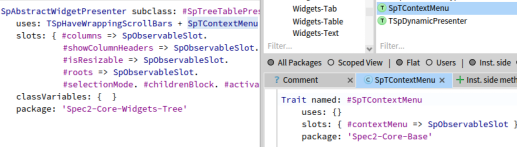
\includegraphics[width=0.5\linewidth]{traits.png}
\end{frame}

\begin{frame}{Optional Green threads}
\begin{itemize}
    \item Pharo includes own process management that allows using concurrent programming even on platforms that do not support it.
\end{itemize}
\begin{block}{}
Built-in Pharo process manager
\end{block}
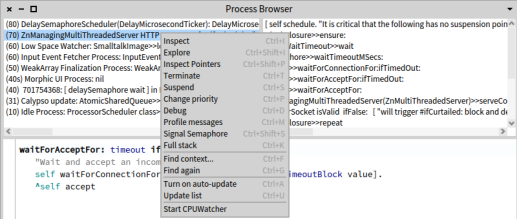
\includegraphics[width=0.5\linewidth]{processes.png}
\end{frame}

\begin{frame}{AST metalinks}
\begin{itemize}
    \item Abstract syntax tree of methods can be extended by metalinks that enable doing additional operations before, after or instead of particular AST nodes. That allows the clean first-class implementation of features like breakpoints, coverage testing, variables that remember old values, etc.
\end{itemize}
 \begin{block}{}
Installation of a breakpoint on an AST node. Example bytecode of a method with breakpoint.
 \end{block}
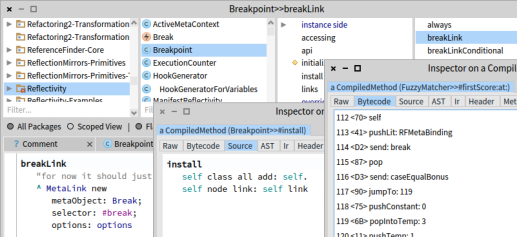
\includegraphics[width=0.5\linewidth]{metalinks.png}
\end{frame}

\begin{frame}{First-class customizable instance variables}
\begin{itemize}
    \item Instance variables described by objects, too. This makes it easy to implement, for example, much smarter instance variables like variables that keep bidirectional managed references between two objects. A simple assignment then automatically updates the other side of the reference, too.
\end{itemize}
\begin{block}{}
Part of a general language meta-model that defines many-to-one relation between package and its owner. When you secify a class package with a simple assignment, the class is added to the child entities collection of the package automatically.
\end{block}
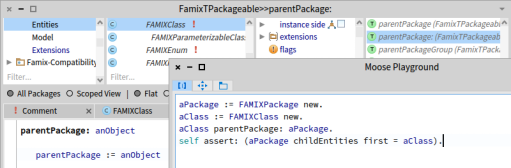
\includegraphics[width=0.5\linewidth]{slots2.png}
\end{frame}

\begin{frame}{Customizable metaclasses}
\begin{itemize}
    \item Objects have classes and classes have classes, too, the metaclasses. These metaclasses have a class, too, and Pharo allows using custom ones. It allows having the implementation of language features like traits as standalone libraries without any direct support in the virtual machine.
\end{itemize}
\begin{figure}
    \centering
    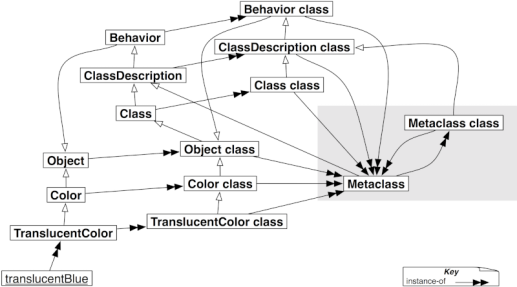
\includegraphics[width=0.5\linewidth]{metaclass.png}
    \caption{Metaclasses}
    \label{fig:metaclass}
\end{figure}

\end{frame}

\begin{frame}{Relatively low memory consumption}
\begin{itemize}
    \item Pharo, including the virtual machine, is very compact with fast startup time.
\end{itemize}
\begin{figure}
    \centering
    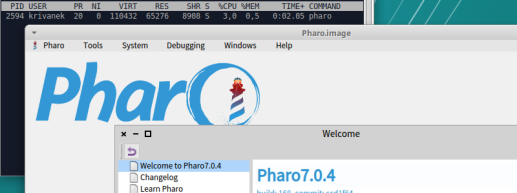
\includegraphics[width=0.5\linewidth]{memory.png}
    \caption{The Pharo IDE in the default configuration consuming 64MB of the physical memory}
    \label{fig:memory}
\end{figure}
\end{frame}

\begin{frame}{Platformski nezavisno korisničko sučelje}
\begin{itemize}
    \item The default Pharo UI looks and behaves the same way on all platforms
    Zadani početni Pharo UI izgleda i ponaša se na isti način na svim platformama
\end{itemize}
\begin{figure}
    \centering
    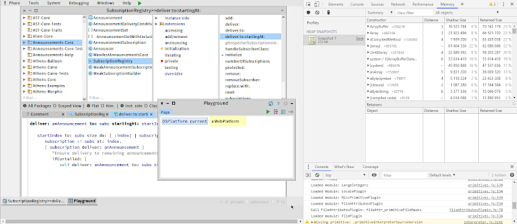
\includegraphics[width=0.5\linewidth]{web.png}
    \caption{Pharo running in a web browser in a virtual machine written in JavaScript. The UI is the very same. Pharo pokrenut u web pregledniku u virtualnom stroju koji je napisan u JavaScriptu. UI je potpuno jednak.}
    \label{fig:web}
\end{figure}
\end{frame}

\begin{frame}{Customizable compiler Prilagodljivi kompajler}
\begin{itemize}
    \item The compiler is written in Pharo, and you can modify it as anything else in the system. You can use completely different compilers for some of your classes.
    Kompajler je napisan u Pharu i možete ga modificirati kao i bilo što drugo u sustavu. Možete koristiti potpuno različite kompajlere za neke od klasa. 
\end{itemize}
\begin{figure}
    \centering
    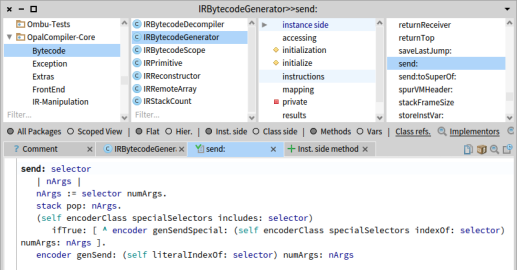
\includegraphics[width=0.5\linewidth]{opal.png}
    \caption{You can browse and modify the compiler on the fly
Možete pregledavati i modificirati kompajler tijekom izvođenja}
    \label{fig:opal}
\end{figure}
\end{frame}

\begin{frame}{Moldable development tools}
%\includegraphics[width=0.5\linewidth]{moldable.gif}
\begin{itemize}
    \item To be more productive, blacksmiths create custom tools for their tasks. Pharo shares the same philosophy. It allows you to create naturally dedicated tools for better understanding of your problems, supporting you in faster development
    \item Write a small simple tool that shows differences between actual and automatically formatted codes inside the Pharo class
\end{itemize}
\begin{block}{}
 Collection
\end{block}
\end{frame}
\begin{frame}{Embedded Animation}
  \animategraphics[loop,controls,width=0.8\linewidth]{17}{moldable/moldable-}{0}{181}
\end{frame}

\begin{frame}{Optional complete object memory persistence}
%\includegraphics[width=0.5\linewidth]{persistence.gif}
\begin{itemize}
    \item All objects in the system can be stored at once in a platform-independent file named image. So you can, for example, save complete state of your program during debugging and restore it to try to find a different execution path or alternative solution.
\end{itemize}
\begin{block}{}
Install a breakpoint, run the application, and when the debugger appears, save the system state. Do some steps inside the debugger and then close Pharo. Recover the saved state and repeat the stepping.
\end{block}
\end{frame}

\begin{frame}{Integrated Git support Ugrađena podrška za Git}
\begin{itemize}
    \item Pharo has advanced integrated Git support that goes beyond the standard level of files. You can merge your branches on the granularity of particular methods, browse their history, create pull-requests directly from the IDE, and so on.
    Pharo ima naprednu integriranu podršku za Git koja nadilazi standardnu razinu datoteka. Možete spajati grane koje imaju zrnatost od nekoliko metoda, pregledati njihovu povijesti, stvoriti pull-requestove direktno iz IDE-a itd. 
\end{itemize}
\begin{figure}
    \centering
    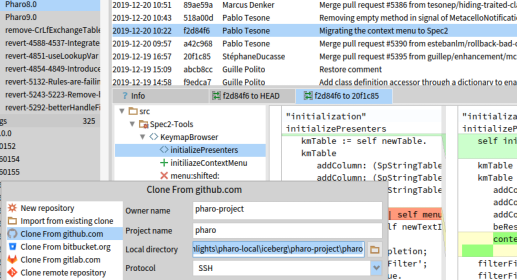
\includegraphics[width=0.5\linewidth]{iceberg.png}
    \caption{The built-in Git manager named Iceberg
Ugrađeni Git manager Iceberg}
    \label{fig:iceberg}
\end{figure}
\end{frame}

\begin{frame}{Fast objects serialization Brza serijalizacija objekata}
All objects, including classes or running contexts, can be serialized to a file. You can, for example, store the state of a debugger with the content of current stack and attach it to the issue report.
Svi objekti, uključujući klase ili kontekst izvođenja, mogu se serijalizirati u datoteku. Može se, na primjer, spremiti stanje debugera zajedno sa trenutnim sadržajem stoga i priložiti ih uz izvješća o poteškoćama. 
Spremanje stoga poziva u datoteku 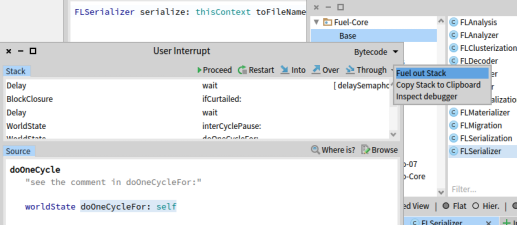
\includegraphics[width=0.5\linewidth]{fuel.png}
\end{frame}

\begin{frame}{Arithmetic precision Aritmetička preciznost}%\includegraphics[width=0.5\linewidth]{numbers.gif}
\begin{itemize}
    \item Pharo can use fractions, scaled decimals, large integers and so on to work with numbers without loss of arithmetic precision.
    Pharo koristi razlomke, skalirane decimale, velike cijele brojeve itd. da bi radio s brojevima bez gubitka aritmetičke preciznosti
\end{itemize}
\begin{block}{}
Pharo and the 0.30000000000000004 problem
\end{block}
\end{frame}


\begin{frame}{Simple connection to native libraries Jednostavno poveziavnje s native knjižnicama}
\begin{itemize}
    \item Pharo includes an FFI interface that makes the creation of bindings to C libraries very straightforward.
    Pharo uključuje FFI sučelje uz koje je stvaranje poveznica na C knjižnice vrlo jednostavno. 
\end{itemize}
\begin{figure}
    \centering
    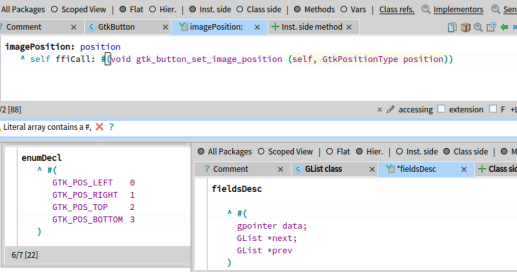
\includegraphics[width=0.5\linewidth]{ffi.png}
    \caption{Part of the GTK binding. The definitions are very natural.
Dio GTK povezivanja. Definicije su vrlo prirodne.}
    \label{fig:ffi}
\end{figure}
\end{frame}

\begin{frame}{Easy use of proxy objects}
\begin{itemize}
    \item Ability to easily create proxy objects - objects that process and/or resend all messages to another object, is essential to object-oriented languages.
\end{itemize}
\begin{figure}
    \centering
    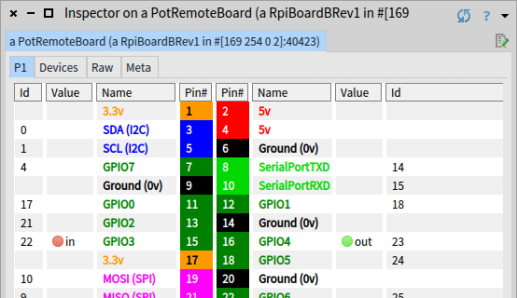
\includegraphics[width=0.5\linewidth]{iot.png}
    \caption{RaspberryPi GPIO ports displayed on a remote Pharo instance }
    \label{fig:iot}
\end{figure}
\end{frame}

\begin{frame}{User interface themes}
\begin{itemize}
    \item Pharo supports custom user interface themes.
\end{itemize}
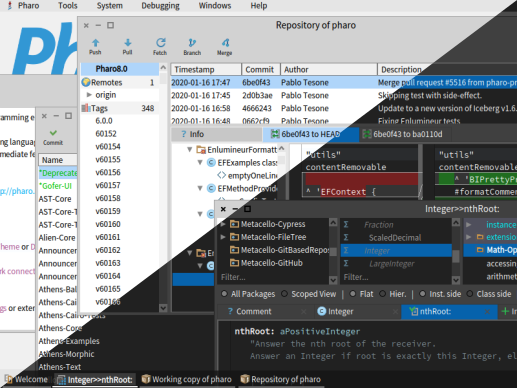
\includegraphics[width=0.5\linewidth]{themes.png}
\begin{figure}
    \centering
    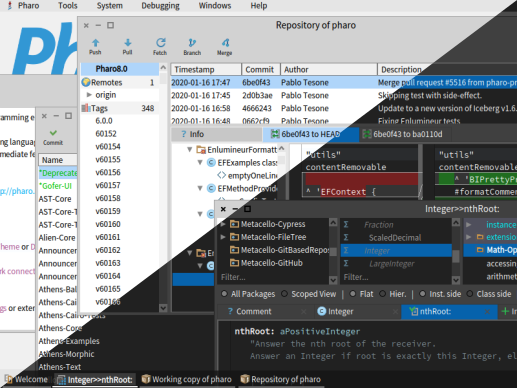
\includegraphics[width=0.5\linewidth]{themes.png}
    \caption{RspberryPi GPIO ports displayed on a remote Pharo instance }
    \label{fig:themes}
\end{figure}
\end{frame}

\begin{frame}{Rigid system nature}
In Pharo, the programmers have almost absolute freedom to customize the system and use many potentially dangerous features. On the other hand, most programmers will use them with deliberation, because Pharo, by default, provides a powerful standard library and tools that shape how to use the system the right way. Instead of making the language strict, it guides the programmers to do things right.
\begin{block}{}
Not all messages are safe to send…
\end{block}
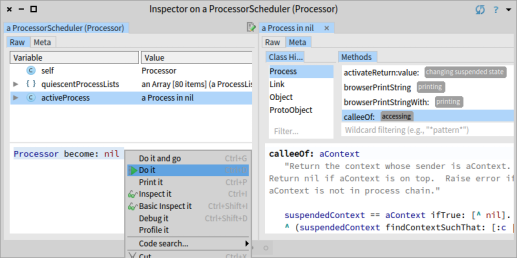
\includegraphics[width=0.5\linewidth]{dangerous.png}
\end{frame}

\begin{frame}{MIT license}

\includegraphics[width=0.5\linewidth]{OSIApproved.png}
\begin{itemize}
    \item Pharo is distributed with a non-viral open-source MIT license.
\end{itemize}
\begin{block}{}
 The main Pharo repository is hosted on GitHub.
\end{block}
\end{frame}

\section{Povijest}
\begin{frame}{Kronologija}
\begin{itemize}
    \item 80-e - Squeak, okruženje otvorenog koda za Smalltalk (Dan Ingalls i Alan Kay)
    \item 16. ožujak 2008. - Pharo, "fork" (grana) Squeaka, S. Ducasse i M. Denker
\end{itemize}
\end{frame}
\section{Usporedba}
\subsection{Python vs. Pharo}
\begin{frame}[fragile]{Simplicity, Conciseness, and Elegance}
Pharo is simpler than Python. It has all of six reserved words. The complete syntax fits on a post card.
You can learn the entire language in 15 minutes: Learn Smalltalk with ProfStef. 
Pharo is astonishingly concise and elegant. Here’s a sampling of wonderful one-liners:

\resizebox{\linewidth}{!}{
\parbox{600px}{
    \ttfamily 
"Compute difference in days between two dates" ('2014-07-01' asDate - '2013/2/1' asDate) days

"Set up an HTTP server that returns the current timestamp"

(ZnServer startDefaultOn: 8080) onRequestRespond: 

[ :request | ZnResponse ok: (ZnEntity with: DateAndTime now printString) ]
    
"Split a string on dashes, reverse the order of the elements and join them using slashes"

\$/ join: (\$- split: '1969-07-20') reverse

"Sum of the primes up to 64" (Integer primesUpTo: 64) sum

"Extract a Unix format timestamp from the 5th to 8th byte of a byte array given in hex"

DateAndTime fromUnixTime:  

((ByteArray readHexFrom: 'CAFEBABE4422334400FF')  copyFrom: 5 to: 8) asInteger
      
"Return the weekday of a date" '2013/5/7' asDate dayOfWeekName

"Save the HTML source of a web page to a file" 'http://www.pharo.org' asUrl saveContentsToFile: 'page.html'

"Count the number of, or show the leap years between two years"

(1914 to: 1945) count: [ :each | Year isLeapYear: each ].

(1895 to: 1915) select: [ :each | Year isLeapYear: each ].

"Encode the same string using Latin1, UTF-8 and UTF-16"

\#(latin1 utf8 utf16) collect: [ :each |  (ZnCharacterEncoder newForEncoding: each)   encodeString: 'Les \'{e}l\`{e}ves Fran\c{c}ais' ]}}
    
In Python, it’s almost impossible to do anything in one line.
\end{frame}
\begin{frame}{Off-side Rule}
Python’s use of indentation as syntax is highly controversial. It’s the main reason why so many developers hate Python. One issue is that an accidental misalignment of code can cause a very subtle and difficult-to-find bug. Who can claim that accidents never happen?
Pharo doesn’t suffer from this malady.
\end{frame}
\begin{frame}{Object-oriented Programming}
Pharo is purely object-oriented from top to bottom. Its clarity and consistency in this regard are unmatched by any other language.
Python, on the other hand, has a makeshift implementation of OOP that feels bolted on. For example, there is no true encapsulation in Python: instance variables and methods are “hidden” or made “private” by prefixing their names with underscores. This is extremely kludgy.
Python requires you to explicitly pass “self” as the first argument to all instance methods. This is unbelievably hokey.
Python objects don’t always have the attribute that you expect. For example, the length property is almost always an external function called len().
\end{frame}
\begin{frame}{Functional Programming}
Pharo has a lovely implementation of lambdas in its “blocks.” This provides Pharo with a nice functional programming capability. In fact, Pharo’s class library contains many functional constructs.
Python can also do functional programming after a fashion. However, its lambdas are restricted to a single expression, rather than allowing for multiple lines of code. No other programming language in the world has this restriction! I hesitate to call this hokey and kludgy. (Okay, I lied: it’s hokey and kludgy.)
\end{frame}
\begin{frame}{IDE (integrated development environment)}
Pharo has a lovely built-in live coding IDE that’s every bit as simple and easy to use as the language itself. Live coding allows you to inspect and modify the code and data in your program while it’s running! This powerful technique practically eliminates the traditional edit-compile-test-debug cycle that has hampered developers for over half a century. This is the main reason why Pharo (Smalltalk) is the most productive general-purpose programming language in the world, according to a study conducted by Namcook Analytics.
Python’s best IDE is PyCharm. While it’s a nice IDE to be sure, there’s no question that it’s much, much larger and more complex than Pharo’s IDE. It would take a long time to master this program.
And PyCharm doesn’t support live coding.
\end{frame}
\begin{frame}{Productivity and Ease of Development}
Python has a reputation for being productive. Namcook Analytics tell us that Pharo (Smalltalk) is twice as productive as Python. This is on average. In many cases, Pharo will be much more productive, sometimes by a factor of five!
Plain and simple, Pharo is just much easier to use for programming. The language and its development environment present virtually no cognitive load on the developer.
\end{frame}
\begin{frame}{Ecosystem}

Python has an enviable ecosystem of libraries. This is a weak point for Pharo. Despite this, Pharo is incredibly versatile. It’s used for many different kinds of applications. For example, Pharo is very good for web development, thanks to the Seaside web framework and the Teapot micro framework.
Pfront-end developmentPharoJS.
data science,  PolyMath  Roassal.
Phvirtual reality:
Internet of Things and embedded programming. See Learn How To Program.

used to script the Unreal game engine:
used to fight Ebola!
used in wide-scale data visualization for medicines in 16 countries.
Pused for natural language processing.
used for machine learning and neural network processing.

Smalltalk, in general, is versatile. The U.S. joint military used Smalltalk to write a million-line battle simulator called JWARS. It actually outperformed a simular program called STORM written in C++ by the U.S. Air Force. 
Smalltalk was used by JP Morgan to write their massive financial risk management system called Kapital.
Orient Overseas Container Lines used Smalltalk to develop their IRIS-2 shipping management system.
If Pharo is disadvantaged by its ecosystem, it certainly doesn’t seem to slow it down. In fact, I think it’s fair to say that Pharo is more versatile than Python.
\end{frame}
\begin{frame}{Multithreading}
Both Pharo and Python can do multithreading, but Python is hampered by the GIL (global interpreter lock), long a complaint of most programmers.
\end{frame}

\section{Sintaksa}

\subsection{Sažetost}
\begin{frame}{Ključne riječi}
    
\resizebox{\linewidth}{!}{
\begin{tabular}{r | l}
\hline
\multicolumn{2}{c}{Samo šest rezerviranih ključnih riječi}
 \\ \hline
\color{red}nil & nedefinirani objekt\\
\color{red}true,false & boolean objekti\\
\color{green}self & objekt primatelj trenutne poruke\\
\color{green}super & objekt primatelj za pristup nadjačanim metodama\\
\color{green}thisContext & trenutno aktivni blok ili metoda\\
\end{tabular}}


\end{frame}
\begin{frame}{Pharo sintaksa na razglednici}
    
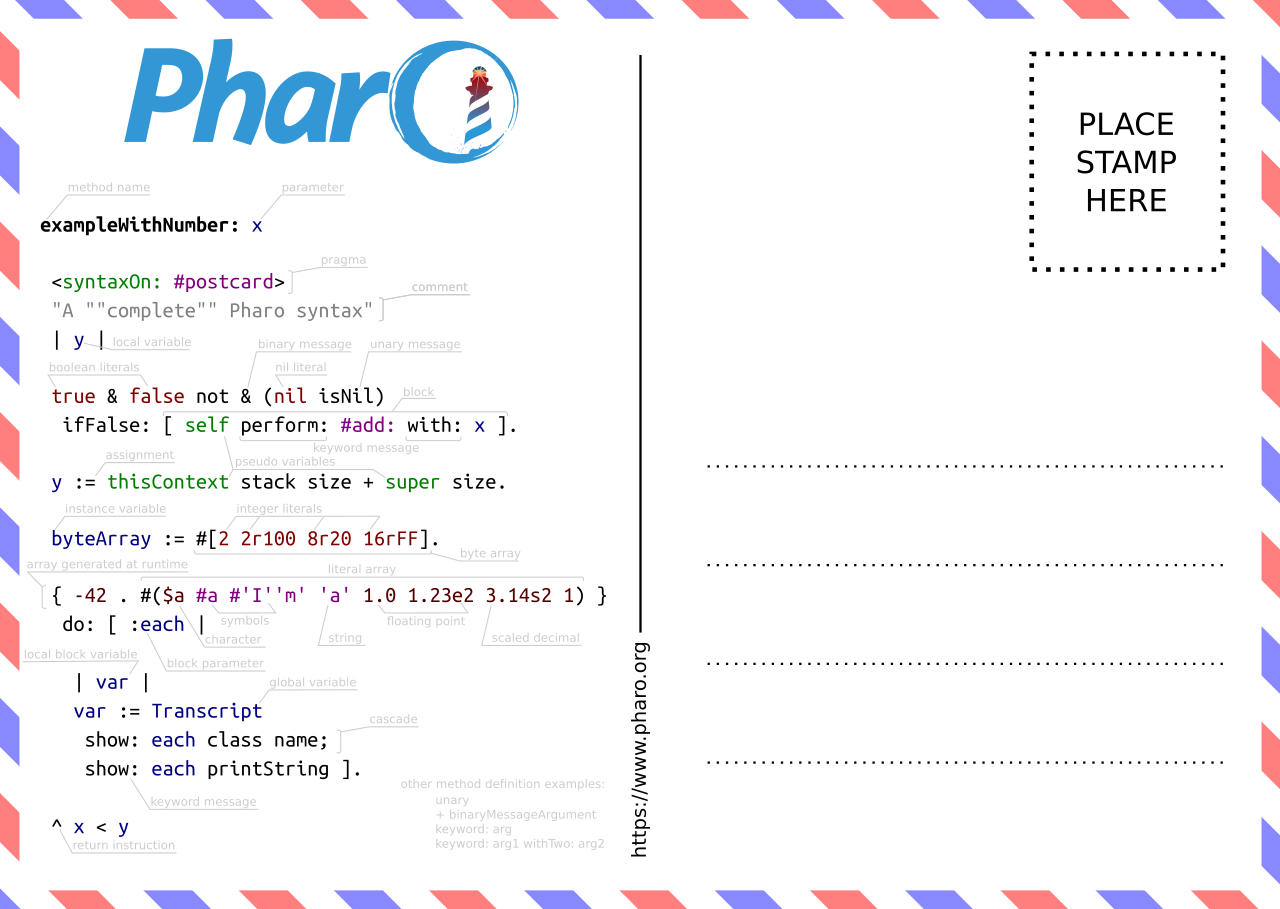
\includegraphics[width=0.95\linewidth]{1280px-Pharo_syntax_postcard.svg.png}

\end{frame}
\subsection{Tipovi podataka}
\begin{frame}{String}

\end{frame}
\begin{frame}{Array}

        \resizebox{\linewidth}{!}{
        \parbox{500px}{
            \ttfamily 
\#[\color{red}123 21 255\color{black}] $\rightsquigarrow$ a ByteArray [3 items] (123 21 255)

\color{black}\#(\color{purple}abc \color{red}123 \color{black}\#[\color{red}1 2 4\color{black}]) $\rightsquigarrow$ an Array [3 items] ('abc' 123 \#[1 2 4])

\color{black}\{ \color{red}2 \color{black} + \color{red}3 \color{black} .   \color{purple}'ab'\color{black}, \color{purple}'cd'\color{black} \}. $\rightsquigarrow$ an Array [2 items] (5 'abcd')}}
\end{frame}
\subsection{Poruke}
\begin{frame}{Binarne i unarne poruke}
Kada šaljemo poruke objektu (primatelju), odgovarajuća metoda se bira i izvršava te odgovara na poruku drugim objektom. Sintaksa poruka oponaš prirodni jezik, sadrži subjekt, predikat i komplemente.

    \begin{itemize}
    
        \item Unarne poruke - \color{red} objekt \color{orange} operator \color{black}
        
        \resizebox{\linewidth}{!}{
        \parbox{500px}{
            \ttfamily 
            \color{red} 1 \color{black} class. $\rightsquigarrow$ SmallInteger
            
            \color{black} false not. $\rightsquigarrow$ true
            
            \color{blue} Date \color{black} today. $\rightsquigarrow$ 2 March 2021
            
            \color{blue} Time \color{black} now. $\rightsquigarrow$ 9:31:18.639933 am
            
            \color{blue} DateandTime \color{black} now. $\rightsquigarrow$ 2021-03-02T09:32:48.691933+01:00
        }}
            
        \item Binarne poruke - \color{red} objekt \color{orange} operator \color{red} drugiObjekt \color{black}
        \resizebox{\linewidth}{!}{ 
        \parbox{500px}{
        
             \ttfamily \color{red} 3 \color{black} * \color{red} 2\color{black}. $\rightsquigarrow$ 6
             
             \color{black} Date today year =  2011. $\rightsquigarrow$ false
             
             \color{black} false  $|$ false. $\rightsquigarrow$ false
             
             \color{black} true \& true. $\rightsquigarrow$ true
             
             \color{black} true \& false. $\rightsquigarrow$ false
             
             \color{red} 10 \color{black} @ \color{red} 100\color{black}. $\rightsquigarrow$ (10@100)
             
             \color{red} 10 \color{black} $<=$ \color{red} 12\color{black}. $\rightsquigarrow$ true 
             
             \color{purple} 'ab'\color{black}, \color{purple} 'cd'\color{black}. $\rightsquigarrow$ 'abcd' }}
    \end{itemize}
\end{frame}
\begin{frame}{Poruke s ključnim riječima}
    \begin{itemize}
        \item Poruke s ključnim riječima (imaju argumente) -
    objekt ključ: drugiObjekt jošJedanKljuč: jošJedanObjekt
    
 
        
Array with: 'hello' with: 2 with: 'Pharo'. $\rightsquigarrow$ an Array [3 items] ('hello' 2 'Pharo')

[ :x | x + 2 ] value: 7 9
    \end{itemize}
\end{frame}
\begin{frame}{Redoslijed izvođenja}
   
\resizebox{\linewidth}{!}{
Zagrade $>$ Unarne poruke $>$ Binarne poruke $>$ Poruke s ključnim riječima 
}

\resizebox{\linewidth}{!}{
\parbox{500px}{
\ttfamily
\color{red} 2.5 \color{black} + \color{red} 3.8 \color{black} rounded. $\rightsquigarrow$ 6.5 

\color{red} 3\color{black} \textbf{ }max: \color{red}2 \color{black} + \color{red} 2\color{black}. $\rightsquigarrow$ 4 
  
(\color{red}0\color{black}@\color{red}0\color{black}) class. $\rightsquigarrow$ Point 

\color{red}0\color{black}@\color{red}0 \color{black} x: \color{red}100\color{black}. $\rightsquigarrow$ 100@0 

(\color{red}0\color{black}@\color{red}0 \color{black} x: \color{red}100\color{black}) class. $\rightsquigarrow$ Point 
}}
Poruke istog prioriteta evaluiraju se zdesna nalijevo

NE VRIJEDI ARITMETIČKI PRIORITET MNOŽENJA I DIJELENJA NAD ZBRAJANJEM
\resizebox{\linewidth}{!}{
\parbox{500px}{
\ttfamily
\color{red}-12345 \color{black} negated asString reversed. $\rightsquigarrow$ '54321' 



\color{red}2 \color{black} + \color{red}2 \color{black} * \color{red}10\color{black}. $\rightsquigarrow$ 40 

\color{red}2 \color{black}+ (\color{red}2 \color{black} * \color{red}10\color{black}). $\rightsquigarrow$ 22 

\color{red}8 \color{black} - \color{red}5 \color{black} / \color{red}2\color{black} \color{black}. $\rightsquigarrow$ 1.5 

(\color{red}8 \color{black} - \color{red}5 \color{black}) / \color{red}2\color{black}. $\rightsquigarrow$ 1.5 

\color{red}8 \color{black} - (\color{red}5 \color{black} / \color{red}2\color{black}). $\rightsquigarrow$ 5.5 
}}
\end{frame}
\end{document}
